
\Section{Introduction}
\label{sec:intro}

In 2002, the Defense Advanced Research Projects Agency (DARPA) High
Productivity Computing Systems (HPCS) program began funding an initiative to
build the next generation of supercomputers, increasing the
performance and productivity of current HPCS architectures by a factor
of 10.

One of the primary goals of the DARPA HPCS Program is to provide a
definition of productivity to evaluate whether vendors have achieved a
10x improvement\cite{Faulk04}.  Current benchmarking mechansims are
performance, rather than productivity based.  For example,
Activity-Based Benchmarks are used to measure system performance
during runtime, typically in floating-point operations per second
(FLOPS).  Unfortunately, this type of benchmark ignores the majority
of effort invested in the development of the software before reaching
the point at which it is ready for execution.

To address the shortcomings of traditional Activity-Based Benchmarks (ABB),
Gustafson et. al. \cite{Gustafson04} proposed the idea of a Purpose-Based
Benchmark (PBB).  A Purpose-Based Benchmark differs from an
Activity-Based Benchmark in that it accounts for all project effort
from its inception (design phase) through to its terminal phase,
which is usually verification/validation and maintenance.  Another
characteristic of PBBs is that each one must model a problem of ``direct
interest to humans'' \cite{Gustafson04}.  For example, a PBB might be
created to accurately predict the weather over the next 3 days or to
simulate the events of an automobile collision.

In this paper, results are presented from an implementation of the
Optimal Truss PBB.  Simply stated, the Optimal Truss problem is
defined as follows:  Given two attachment points on a vertical surface
and a load-bearing point some distance from that surface, find a
pin-connected, steel truss structure that uses as little mass as
possible to bear the load with a safety factor of 50 percent.  An initial
implementation of the Optimal Truss PBB was composed over the Spring of
2004 and is used as a basis of data for results in this paper.  More
details about the Optimal Truss PBB appear in Section 4.

Concurrently with the development of the Optimal Truss PBB, I gathered
software engineering data for each day of development on the PBB in
the form of Hackystat\cite{HackySite} diaries and journal entries.
Hackystat is a tool that provides software developers with automated
support for collecting and analyzing useful measures of the process
and products of software development.  The Hackystat diaries are
automatically constructed from activities that take place within an
editor (e.g. Emacs or Vim).  Hackystat sensors for these tools collect
activity data and send it to a Hackystat server for storage and
analysis.  The journal entries I compiled during PBB development were
personal, handwritten entries reflecting on processes or products that
I felt Hackystat did not capture.

One of the primary reasons for maintaining the software engineering
data related to the Optimal Truss PBB was to gain insight into time
allocation of HPCS developers.  In order to realize productivity
gains, one must first understand where the bottlenecks exist.
Specifically, it is important to characterize active time between the
``sequential'' aspects of development and those that are considered
``parallel''.  For example, the workflow of an HPCS developer might be
classified into the general categories:

\begin{enumerate}
  \item {\bf Developing the sequential workhorse} - this typically
  involves the translation of algorithms and mathematics from model to
  source code.  A sequential workhorse is essentially the unit of
  computation that requires enough execution time to justify the
  latency when communicating its result between two or more nodes.
  For example, in the Truss PBB, one sequential workhorse is solving
  the forces for each joint in the truss.
\item {\bf Parallelizing the sequential
  workhorse} - this typically involves task distribution and
  communication handling for multiple nodes.  For example, in the
  truss PBB, this includes determining which units of computation
  should be sent to which nodes, when the communication should take
  place and when the results should be collected.
\end{enumerate}

One of the funtamental goals of this research is to produce a metric
that classifies the ratio between ``sequential'' and ``parallel''
active time, on a per file basis to isolate and identify bottlenecks,
which can then be addressed and corrected to increase overall
productivity in future projects.

Therefore, from the experience of developing a PBB on a full scale HPCS
architecture and the software engineering data gathered automatically
by Hackystat diaries and manually through personal journals, I propose
a two-part thesis claim that:
\\
\\
1. The software engineering of HPCS systems can be improved by
understanding the way programmers allocate their time between the
``parallel'' and ``sequential'' aspects of a software implementation.
\\
\\
2. A metric can be defined to measure the ratio between the degree of
parallelism and active time of HPCS source code.  This metric will
provide a developer or project manager with a categorization of active
time spent between parallel and sequential development.  This metric
will be defined through an analysis of developer workflow and the
incorporation of automatic tool support.

\Section{Methodology}
\label{sec:methodology}

To evaluate the thesis claims made in the previous section, I plan to
perform an analysis of the software engineering data gathered during
the implementation of the Optimal Truss PBB.  Specifically, I intend
to characterize my own workflow as falling into one of two possible
categories of development, either ``parallel'' or ``sequential''.
Using a combination of the active time data from Hackystat diaries and
self reported time in the developer journals, I intend to create a
time chart indicating the time spent on each portion, on a per file
basis.  For example, if the file ``seq\_workhorse.cc'' is determined
to be ``sequential'', I will credit the sequential portion with the
active time reported in the Hackystat diaries and developer journals.

Once I have performed this analysis on each file, I will be able to
create an initial ratio of active time allocated between ``parallel''
and ``sequential'' development.  I will also be able to identify
potential productivity bottlenecks, by uncovering the files that
required a disproportionate amount of active time.

In parallel with the data analysis, I plan on building a tool to
classify whether a file of source code is ``parallel'' or not.  As an
initial pass, I will designate a ``parallel'' file as one that
contains one or more MPI constructs.  This tool can be achieved by
extending a C++ parser or tokenizer to gather the name and count of
MPI constructs appearing in the source code.

After the tool is built, I hope to integrate it with Hackystat to
couple the degree of parallelism (e.g. whether file is parallel) with
the Hackystat active time analysis.  This should produce a ratio
similar in definition to the one produced manually, but this will be
automatic with little overhead.

With the tool support in place, I hope to apply it to future HPCS
development of my own and in other student environments to
characterize workflow and suggest productivity bottlenecks.

\Section{Collecting Degree of Parallelism/Active Time Metric}
\label{sec:dopatmetric}
In order to define a metric that measures the ratio between active
time spent in parallel and sequential development, it is first
necessary to explain the factors involved.  This includes describing
how a file can be categorized as either ``parallel'' or
``sequential''.  It also involves defining what ``active time'' is in
relation to the file.

In the Truss PBB case study, the code was written primarily in the C++
programming language using libraries provided by the Message Passing
Interface\cite{MPISite} (MPI) to achieve interprocess communication
between nodes in the system.  Files utilizing the MPI libraries have
at least one occurence of an MPI construct.  An MPI construct is
either a call to an MPI function or global variable.  For example,
MPI\_Send and MPI\_Recv are the function names, respectively, for
sending and receiving data between two or more nodes and
MPI\_COMM\_WORLD is the global variable defining which nodes in the
system are available for communication.  

Since here are other message passing libraries available, such as
OpenMP\cite{OpenMPSite} or JavaParty\cite{JavaPartySite}, I will use
the term {\bf parallel construct} to describe any construct involving
message passing among multiple nodes and the term {\bf MPI construct}
to indicate those functions or global variables specific to the MPI
library.  Essentially, MPI constructs are a particular subset of all
available parallel constructs.

To distinguish between a ``parallel'' and ``sequential'' file, one
must parse the source code for occurences of parallel constructs.
Files that contain parallel constructs can be described as being
inherently parallel, as parallel constructs indicate that the file
contains instructions to perform interprocess communication among two
or more nodes.  Therefore, for the Truss PBB implementation which uses
MPI solely for message passing, a ``parallel'' file is one that
contains at least one MPI construct.  It then follows that a
``sequential'' file is one that is absent of any MPI constructs.
Furthermore, we propose a binary relationship for the degree of
parallelism, such that ``parallel'' files have a DOP equal to 1 and
``sequential'' files have a DOP equal to 0.  This definition of degree
of parallelism is source code specific and differs from the industry
definition, meaning the number of nodes involved in the computation,
which is application specific.

In order to automatically categorize source files and determine their
degree of parallelism, I developed an extension to the Lines Of Code
Counter (LOCC) tool developed in the Collaborative Software
Development Laboratory (CSDL) at the University of Hawaii to perform
this task.  LOCC is a grammar-based, heirarchical code-counter that
parses source code to statically extract metrics, such as lines of
code, number of methods, etc.  To obtain the degree of parallelism
metric, I extended LOCC to tokenize the C/C++ programming language and
produce MPI metrics in addition to the existing metrics.  MPI metrics
measure the number of occurences of MPI constructs on an individual
basis.  An example of the LOCC output for a file containing MPI
constructs appears below.

\pagebreak
\begin{figure}
  \includegraphics[width=0.5\textwidth]{locc_output.eps}
  \caption{LOCC metric output including MPI constructs}
  \label{fig:LOCCOutput}
\end{figure}

To create the ratio of source code DOP to active time, it is also
important to understand what is meant by active time and how it is
measured.  For this research, active time is the measurement of time
spent actively editing a file.  To implement this metric, I have
employed the services of the Hackystat tool to gather it automatically
without developer intervention.  The Hackystat system provides sensors
that run unobtrusively in the background of IDE processes, recording
activities and gathering multiple developer metrics, including active
time, which are then sent to a Hackystat server for permanent storage
and analysis.

It is anticipated that the marriage between the LOCC tool and the
Hackystat system will provide the data and analyses to aid a developer
or project manager in understanding time allocation between
``parallel'' and ``sequential'' components.  Below is a sample graph
that illustrates an example of time allocation.

\begin{figure}[h]
  \includegraphics[width=0.5\textwidth]{DOP_ratio.eps}
  \caption{Parallel and serial files trend over time}
  \label{fig:DOPRatio}
\end{figure}
\pagebreak